\documentclass[11pt]{article}

% ---------------------------------------------------------------------------
% Build switch.  \anonfalse = named preprint (arXiv).
%                \anontrue  = anonymised build for CHIL double-blind review.
% ---------------------------------------------------------------------------
\newif\ifanon
\anonfalse

\usepackage[a4paper,margin=2.5cm]{geometry}
\usepackage{times}
\usepackage[T1]{fontenc}
\usepackage[utf8]{inputenc}
\usepackage{amsmath,amssymb}
\usepackage{booktabs}
\usepackage{graphicx}
\usepackage{caption}
\usepackage{authblk}
\usepackage[hidelinks]{hyperref}
\usepackage{xurl}
\usepackage{microtype}
\usepackage[numbers,sort&compress,square]{natbib}

\captionsetup{font=small,labelfont=bf}
\setlength{\parskip}{0pt}
\renewcommand{\arraystretch}{1.12}

\title{\vspace{-1.5em}\bfseries Character accuracy conceals numerical error:\\
silent value corruption in a clinical document pipeline,\\
and what actually prevents it}

\ifanon
  \author[ ]{}
  \affil[ ]{\small Author details withheld for double-blind review}
\else
  \author[ ]{Mohammed Jabir Hussain Shaik}
  \affil[ ]{\small School of Electronics, Electrical Engineering and Computer Science\\
  Queen's University Belfast, United Kingdom\\
  \texttt{mshaik01@qub.ac.uk}}
\fi
\date{}

\begin{document}
\maketitle

\begin{abstract}
\noindent
\textbf{Background:} Clinical decision support systems increasingly read patient data from
document images. Accuracy for that stage is reported at character level, and a laboratory value
is not a character.

\noindent \textbf{Methods:} We measured the image-to-value path of a retrieval-based clinical
decision support prototype under controlled image degradation, using synthetic reports carrying
exact machine-readable ground truth, with the document as the experimental unit. Four
experiments covered 2{,}820 values: a degradation sweep, a resolution study replicated across 10
reports, a comparison of seven recognition approaches including a fine-tuned recogniser, and an
evaluation of four verification checks. Held-out testing used 20 further reports typeset in
fonts no model had seen.

\noindent \textbf{Results:} At 100~dpi, character accuracy remained at 88.9\% while 32.3\% of
laboratory values were misread. Of 188 corrupted values, 89 (47.3\%) carried the same
abnormality flag as the truth and so were invisible to the alerting layer. Because flags are
threshold quantisations, corruption of an already-abnormal value was more often silent than
corruption of a normal one (61.7\% against 22.1\%; risk ratio 2.80, 95\% CI 1.75--4.47), an
effect that held with the document as the unit of analysis (paired difference 43.0 percentage
points, $p = 0.0078$). Fine-tuning the recogniser did not help: it read the document it was
tuned for perfectly at low resolution but was no better than the stock model on held-out reports
($p = 0.63$). Upscaling the page before recognition was the largest single gain, improving
low-resolution accuracy from 60.0\% to 98.5\%. A vision--language model transcribed legible
pages accurately but, on degraded pages, produced fluent values that were not printed and moved
them toward the normal range. Requiring agreement between two independently built readers caught
193 of 193 corruptions on held-out data at a 19.8\% review rate.

\noindent \textbf{Conclusions:} Character-level accuracy is not a safety metric for pipelines
that reduce measurements to flags, and the errors such pipelines hide fall disproportionately on
patients whose values are already abnormal. In the conditions tested, verification by a second
independent reader reduced undetected errors more than any improvement to the recogniser itself.
All findings come from synthetic documents and bound no claim about performance in deployment.
\end{abstract}

\section{Introduction}

A clinical decision support system that reads a patient record from a scanned page performs a
chain of inferences before any model reasons about the patient. Pixels become characters,
characters become a labelled value, the value is compared against a reference range, and the
resulting flag reaches the clinician or the generator. Each step can fail, and the failures do
not announce themselves in the same way.

Work on retrieval-augmented generation in healthcare has concentrated on what happens after a
value exists: whether the right passage is retrieved, whether the answer is grounded, whether a
citation points where it claims to \citep{gao2023rag,amugongo2025rag,lu2024clinicalrag}. That
literature assumes the number arriving from the document is the number printed on it. When the
document is a photograph or a fax, the assumption is doing work that nobody has measured.

Optical character recognition is normally reported through character error rate, and character
error rate treats every symbol as equivalent. A decimal point is one character. In
\texttt{5.8 mEq/L} it is also the difference between a potassium concentration requiring
monitoring and one incompatible with life. A pipeline can therefore post a high character
accuracy and still deliver a wrong number, and the number is what the clinical logic consumes.

The clinical stakes are concrete. Laboratory results reach clinicians as scanned or faxed
documents in many settings, including transfers between institutions, referrals from primary
care, and any workflow where a patient carries paper from one provider to another
\citep{wang2026keycoverage}. A decision support system that reads such a document and returns a
treatment suggestion has already made a measurement before it makes an argument. If the
measurement is wrong and nothing downstream can tell, the system is confidently wrong in a way
its own confidence scores will not reveal.

We state the boundary of this work at the outset. Everything reported here was measured on
synthetic reports generated with exact machine-readable ground truth, which is what makes
value-level error measurable at all and what makes it impossible to claim a rate for any
deployed system. No real patient record was processed, no clinician assessed any output, and no
clinical decision or patient outcome was simulated or measured. What follows is a measurement of
software behaviour under controlled image degradation, and should be read as establishing the
existence and mechanism of a failure mode rather than its prevalence in practice.

We report four experiments on this path. The first sweeps 32 degradation conditions on a single
document to establish which corruptions occur. The second takes the document as the
experimental unit across 10 independent reports and 7 resolutions, and measures how often
values are misread, how often they are lost, and what the system's own flagging layer does with
the result. The third asks whether a better reader fixes the problem, comparing seven
recognition approaches, including a recogniser we fine-tuned on synthetic laboratory lines, on
both the original document and a held-out set of reports typeset in fonts the fine-tuned models
never saw. The fourth asks what catches the errors that remain.

Our contributions are the following. We quantify the dissociation between character accuracy
and value accuracy in a clinical extraction pipeline. We give a taxonomy of what corruption
does to an abnormality flag, and show that the most common outcome is no change at all. We
identify the mechanism behind that outcome, which is threshold quantisation, show that it is
predicted by whether the true value was already abnormal, and analyse it with the document as
the experimental unit so that the effect does not rest on treating readings from one page as
independent. We evaluate a physiological plausibility bound and characterise where it
systematically fails, and we report that replacing the deterministic extractor with a language
model repaired no error and introduced none. We then show that fine-tuning the recogniser is not
the remedy it appears to be, that a preprocessing change outperforms it on unseen material, that
a vision--language model substitutes plausible invented values for illegible ones in a direction
that moves results toward normality, and that requiring agreement between two independently
built readers left no undetected wrong value in either test set.

\section{Related work}

\paragraph{Retrieval-augmented clinical systems.}
Retrieval-augmented generation has been proposed widely for clinical question answering, and
recent reviews survey its use across healthcare tasks \citep{gao2023rag,amugongo2025rag}.
Systems such as ClinicalRAG retrieve over heterogeneous clinical knowledge
\citep{lu2024clinicalrag}, and question-answering corpora such as MedQuAD provide evaluation
material \citep{benabacha2019medquad}. These evaluations measure retrieval and generation
quality on text that is already text, and assume the number arriving from the document is the
number printed on it.

\paragraph{Recognition quality and what depends on it.}
Tesseract, the engine measured here, recognises text with an LSTM line model operating on
segmented lines \citep{smith2007tesseract}. Recognition error is conventionally summarised at
the character level, and the limitations of that summary are recognised in the document analysis
literature: Hemmer et al.\ observe that recognition errors degrade downstream natural language
processing and that some are not resolvable from the image even by a human reader
\citep{hemmer2024confidence}. Work on extraction from scanned clinical reports has argued that
accuracy alone is an insufficient criterion, because information lost at the representation
layer never reaches the structured output at all \citep{wang2026keycoverage}. Most directly, Yu et al.\ benchmarked
language-model extraction tools on medical documents and assessed the image distortions
commonly introduced by fax machines, finding a significant impact on extraction performance
\citep{yu2026benchmark}. That result concerns extraction accuracy; the question we take up is
what becomes of such an error once the extracted number has been reduced to a flag.

What this literature measures is how recognition quality affects extraction quality. Yu et al.\
establish that fax-type distortion degrades extraction from medical documents
\citep{yu2026benchmark}; Wang et al.\ establish that information absent from the representation
cannot be recovered downstream \citep{wang2026keycoverage}. Both stop at the extracted field.

\paragraph{Abnormality flags and what they hide.}
A separate literature studies the flags themselves, and studies them from the opposite
direction. Kilickaya and colleagues showed that standard reference ranges derived from healthy
adults mark too many results abnormal in critically ill patients, producing false positive
alerts and alert fatigue, and that customised ranges reduce them \citep{kilickaya2014ranges}.
That work treats the flag as over-sensitive. We report the complementary failure: when the
value reaching the flag is already wrong, the same threshold structure makes a predictable
subset of those errors produce no alert at all. The two findings are consistent, since both
follow from a threshold discarding the distance between a value and its boundary.

Our contribution begins one step later. We ask what happens to a numerical error \emph{after}
extraction, once the value has been compared against a reference range and reduced to an
abnormality flag, and we show that this reduction is itself an information-destroying operation
that hides a predictable subset of errors. To our knowledge the specific result, that
corruption of an already-abnormal value is several times more likely to be invisible than
corruption of a normal one, and the structural reason for it, have not been reported. The
second contribution is the comparative one: that the obvious remedy of fine-tuning the
recogniser does not generalise, while rescaling and cross-reader agreement do. We are not aware
of a prior comparison of these three strategies on the same clinical extraction task with
held-out typography.

\paragraph{Generative readers and confabulation.}
Vision--language models are increasingly used for document understanding, and the risk that a
generative reader produces fluent output unsupported by the source is well recognised. In
enterprise document extraction, adding a governance layer of validation and consistency checking
has been reported to reduce the hallucination rate from 15.7\% to 3.2\%
\citep{sediqin2026sage}. Our observation is the clinical specialisation of the same problem: the
invented values are physiologically ordinary and biased toward normality, which defeats checks
that inspect the value in isolation.

\paragraph{Reporting standards.}
Reporting guidance for clinical prediction and machine-learning models now asks explicitly for
the data pipeline and its failure modes to be described \citep{collins2024tripodai}. This study
is a measurement of one such pipeline rather than a model development study, and we follow that
guidance where it applies by reporting the extraction stage as a source of error in its own
right.

\section{Methods}

\subsection{Documents and ground truth}

Each synthetic report is generated with a machine-readable truth file recording the exact value,
unit, printed reference range and expected flag for 13 analytes: fasting glucose, HbA1c,
haemoglobin, ferritin, white cell count, platelets, sodium, potassium, blood urea nitrogen,
creatinine, eGFR, troponin I and LDL cholesterol. The panel was chosen to span several orders of
magnitude and several decimal conventions, so that a lost decimal point produces an error of
different size depending on the analyte.

No real patient data were used at any stage.

\subsection{Degradation conditions}

Documents are rendered from PDF at a specified resolution and then degraded. The condition set
covers resolution (300, 200, 150, 120, 100, 85 and 72 dpi), Gaussian blur
($\sigma \in \{0.5, 1.0, 1.5, 2.0, 3.0\}$), JPEG compression (quality
$\in \{90, 70, 50, 30, 15\}$), rotation ($\{0.25, 0.5, 1.0, 2.0, 5.0\}$ degrees), additive
noise ($\{5, 10, 20, 30, 50\}$), and five composites intended to resemble real capture paths:
a good scan, an office scan, a phone photograph, a poor fax and a poor photograph.

Stochastic conditions are run with five seeds. Experiment~1 therefore comprises 24
single-seed conditions and 8 conditions at five seeds each, giving 64 runs and, across 13
analytes, 832 observations on one document.

\subsection{Extraction, flagging and the plausibility bound}

Degraded images are passed to Tesseract (\texttt{--psm 6}). A deterministic parser locates each
analyte by label and extracts the first numeric token on the line.

The flagging logic is transcribed, rather than imported, from the prototype's
\texttt{clinical\_parser} module so that the experiment runs without the application stack. The
transcription preserves a property of the deployed system worth stating plainly: its reference
ranges are fixed, are not age- or sex-aware, and are not the ranges printed on the document. The
system flags haemoglobin outside 12.0--17.5~g/dL while the generated
report prints 12.0--15.5~g/dL.

Two properties of this flagging logic matter for interpreting every result below. First,
abnormality is decided against \emph{hardcoded} ranges held in the prototype, not against the
range printed on the document, and the two can differ: the system flags haemoglobin outside
12.0--17.5~g/dL while the generated report prints 12.0--15.5~g/dL. Second, those ranges are
fixed and are neither age- nor sex-aware, and units are assumed rather than parsed, so a change
of unit on the page would not be detected. These are properties of the deployed prototype, and
we preserve them deliberately rather than correcting them, because the object of study is the
pipeline as built. A system using document-printed ranges and parsed units would be exposed to a
different, and in some respects smaller, version of the failure we describe.

We additionally implement a physiological plausibility bound, a generous envelope of values
possible in a living patient, and ask whether it would have rejected each corruption. This
envelope is our own construction for this study, is not a clinical standard, and is not
validated against any laboratory's own limits.

\begin{figure}[t]
\centering
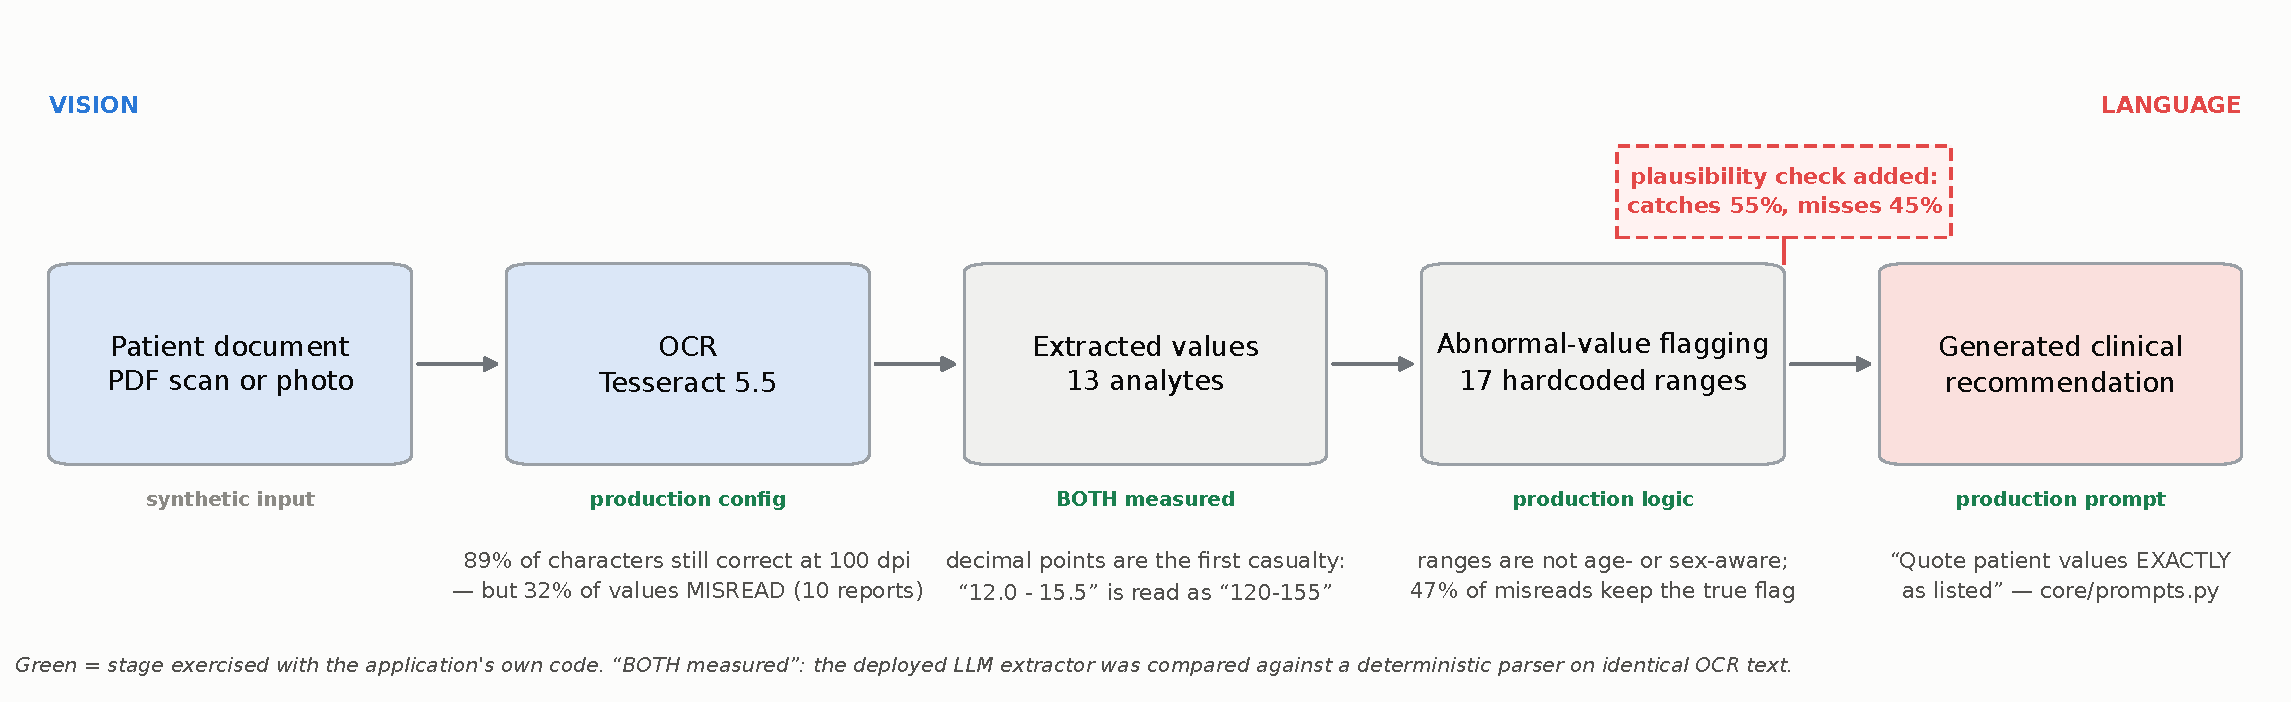
\includegraphics[width=\textwidth]{figures/fig1_architecture.pdf}
\caption{The measured path, with one observed case. A potassium concentration of
5.8~mEq/L printed on the page is extracted as 58.0 and carries the same \emph{High} flag as the
true value. Stages marked in green were exercised using the prototype's own code. The
potassium case is one observed instance from the single-document sweep and is not a frequency.
Whether a corrupted value changes a generated recommendation was not tested.}
\label{fig:pipeline}
\end{figure}

\subsection{Experimental unit and the calibration gate}

Thirteen analytes read from one page are not thirteen independent observations, since they share
a rendering, a scan and an OCR pass. Experiment~2 therefore treats the document as the
experimental unit: proportions are computed within each of 10 independent reports and summarised
across them, and every dispersion we report is a standard deviation between documents rather
than a confidence interval.

No result is reported for a document unless its clean 300~dpi render returns all 13 values
correctly. This gate separates degradation effects from generation or parsing faults. All 10
documents passed.

Experiment~2 comprises 10 documents $\times$ 7 resolutions $\times$ 13 analytes, giving 910
observations.

\subsection{Outcome definitions}

Each reading is \emph{correct}, \emph{misread} (a value was emitted and it differs from truth)
or \emph{unread} (no value was emitted for that analyte). Misread and unread are different
failures with different consequences and we never pool them.

Character error rate is Levenshtein distance between the whitespace-normalised reference text
and the OCR output, divided by the length of the reference.

\section{Results}

\subsection{Which degradations corrupt values, and which destroy them}

Experiment~1 sweeps 32 conditions on one document to establish which failure modes exist before
committing the replicated design to a single axis. Table~\ref{tab:families} gives the outcome by
degradation family.

\begin{table}[t]
\centering
\caption{Experiment~1: outcome by degradation family, 832 observations on one document.
\emph{Corrupted} means a wrong value was emitted; \emph{label not found} means the analyte's line
was not located at all. JPEG compression to quality 15 and rotation to five degrees produced
neither outcome.}
\label{tab:families}
\small
\begin{tabular}{lcccc}
\toprule
Family & Observations & Corrupted (\%) & Label not found (\%) \\
\midrule
Baseline (300~dpi) & 13  & \phantom{0}0.0 & \phantom{0}0.0 \\
JPEG quality 90--15 & 65  & \phantom{0}0.0 & \phantom{0}0.0 \\
Rotation 0.25--5$^\circ$ & 65  & \phantom{0}0.0 & \phantom{0}0.0 \\
Noise 5--50 & 325 & \phantom{0}1.5 & 20.0 \\
Blur $\sigma$ 0.5--3.0 & 65  & \phantom{0}9.2 & \phantom{0}0.0 \\
Composite capture paths & 221 & \phantom{0}6.3 & 56.1 \\
Resolution 200--72~dpi & 78  & 23.1 & 10.3 \\
\bottomrule
\end{tabular}
\end{table}

The families separate by failure mode. Resolution is the dominant source of wrong values.
Noise and the composite capture paths mostly prevent the analyte's label from being located, so
the value is absent rather than wrong. JPEG compression and small rotations produced no error of
either kind at the levels tested.

This distinction matters for risk. An analyte that is not found is an absence a caller can
detect. A misread analyte is a confident wrong answer. Because resolution is the condition that
most readily produces the second case, Experiment~2 replicates the resolution axis across 10
independent documents.

\subsection{Character accuracy and value accuracy separate}

Table~\ref{tab:resolution} gives both measures across the resolution sweep. At 300~dpi no
value was misread in any of the 130 analyte readings. Degradation then affects the two measures
at different rates. Between 300~dpi and 100~dpi, character accuracy falls by
9.2 percentage points while the misread rate rises from zero to 32.3\%.

\begin{table}[t]
\centering
\caption{Character accuracy and value outcomes across the resolution sweep. Each cell is the
mean over 10 independent documents, with the standard deviation between documents in
parentheses. Misread means a wrong value was emitted; unread means no value was emitted.}
\label{tab:resolution}
\small
\begin{tabular}{lccc}
\toprule
Resolution & Character accuracy (\%) & Values misread (\%) & Values unread (\%) \\
\midrule
300~dpi & 98.10 & \phantom{0}0.00 \phantom{(00.00)} & \phantom{0}0.00 \phantom{(00.00)} \\
200~dpi & 98.02 & \phantom{0}1.54 (3.24) & \phantom{0}0.00 \phantom{(00.00)} \\
150~dpi & 96.67 & \phantom{0}4.62 (5.38) & \phantom{0}0.00 \phantom{(00.00)} \\
120~dpi & 96.12 & 12.31 (9.73) & \phantom{0}0.00 \phantom{(00.00)} \\
100~dpi & 88.88 & 32.31 (9.46) & 10.00 (5.19) \\
85~dpi  & 80.83 & 49.23 (13.66) & 14.62 (5.68) \\
72~dpi  & 56.53 & 44.62 (21.08) & 41.54 (27.43) \\
\bottomrule
\end{tabular}
\end{table}

\begin{figure}[t]
\centering
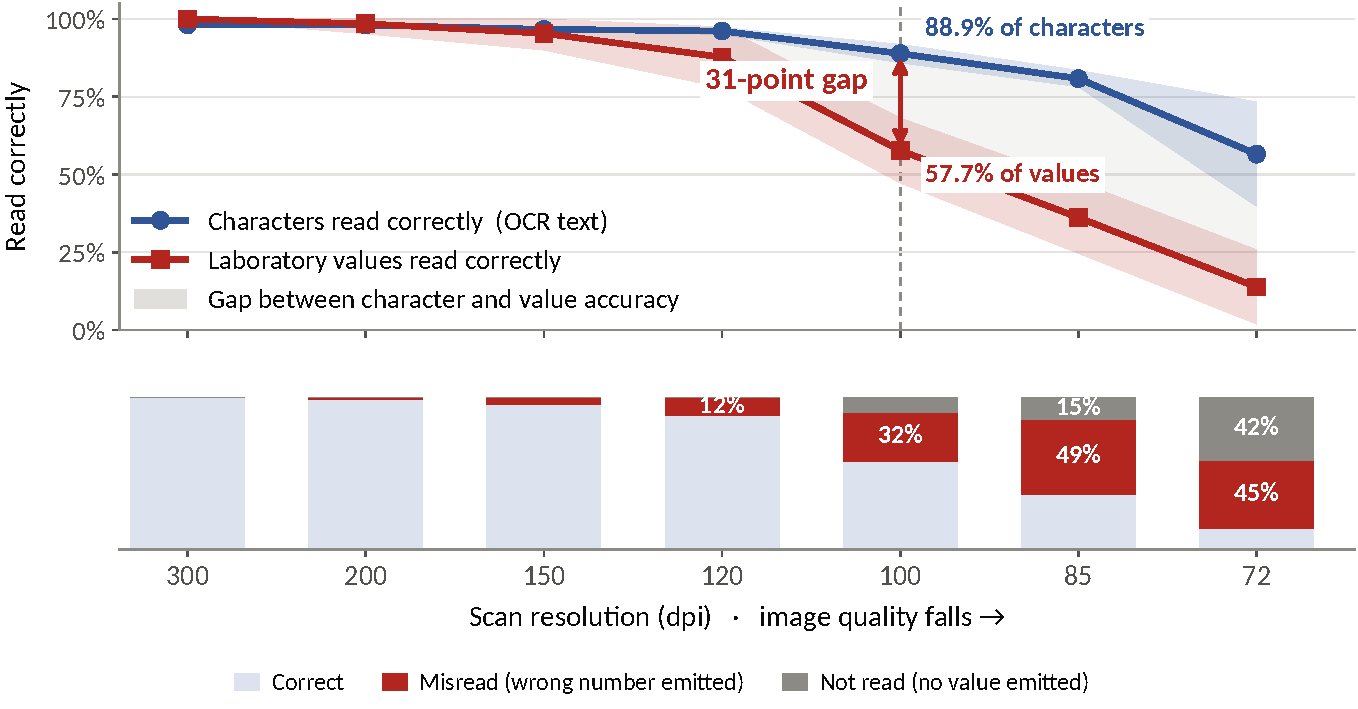
\includegraphics[width=\textwidth]{figures/fig2_resolution_paper.pdf}
\caption{Character accuracy and value accuracy across the resolution sweep. Each point is the
mean over 10 independent documents and bands are $\pm1$ standard deviation between documents,
not confidence intervals. The lower panel decomposes each resolution into values read correctly,
values misread, and values not read. At 100~dpi the two measures differ by 31 percentage points.}
\label{fig:resolution}
\end{figure}

Below 85~dpi the misread rate stops rising while the unread rate more than doubles. Paired
by document between 85~dpi and 72~dpi, the misread rate fell for four documents, rose
for three and was unchanged for three (mean change $-4.6$ percentage points, SD 20.9). The data
are consistent with values ceasing to be read rather than being read wrongly, and they do not
establish a decrease.

\subsection{What corruption does to the flag}

Across Experiment~2, 188 of 910 readings were misread. Table~\ref{tab:taxonomy} classifies each
by what happened to the abnormality flag. The largest category is no change: 89 corruptions
(47.3\%) produced a value that carried the same flag as the truth. For those
readings the error is invisible to any component that consumes the flag rather than the value.

\begin{table}[t]
\centering
\caption{What corruption did to the abnormality flag, for all 188 misread values in
Experiment~2. Categories are mutually exclusive. The silent share computed within each document rather than pooled gives a mean of 48.2 percent (SD 12.7, range 23 to 64 across the 10 documents).}
\label{tab:taxonomy}
\small
\begin{tabular}{lcc}
\toprule
Outcome & Count & Share of corruptions (\%) \\
\midrule
Flag unchanged (silent)                 & 89 & 47.3 \\
Normal value flagged abnormal           & 53 & 28.2 \\
Flag changed, wrong direction or severity & 41 & 21.8 \\
Abnormal value read as normal           & \phantom{0}5 & \phantom{0}2.7 \\
\midrule
Total                                   & 188 & 100.0 \\
\bottomrule
\end{tabular}
\end{table}

\subsection{Already-abnormal values hide their own corruption}

The silent category is not distributed at random. Splitting the 188 corruptions by whether the
true value was already outside its reference range gives 61.7\% silent (95\% CI 52.7--69.9)
among the 120 corruptions of abnormal values, against 22.1\% (95\% CI 13.8--33.3) among the 68
corruptions of normal values (Figure~\ref{fig:mechanism}; Fisher exact
$p = 1.6 \times 10^{-7}$). Because corruption is a common outcome in both groups, the odds ratio
of 5.68 overstates the multiplicative effect and we report the risk ratio instead: corruption of
an already-abnormal value was 2.80 times as likely to be silent (95\% CI 1.75--4.47), a risk
difference of 39.6 percentage points.

That test assumes the 188 corruptions are independent, and they are not: they are clustered
within 10 documents and 13 analytes, and corruptions sharing a document also share a rendering
and an OCR pass. We therefore repeat the comparison with the document as the unit of analysis.
Eight of the 10 documents produced corruptions of both abnormal and normal values. Within those
eight, the silent share is 65.3\% (SD 17.3) for corruptions of abnormal values against 22.3\%
(SD 20.1) for corruptions of normal values, a paired difference of 43.0 percentage points
(SD 24.3; Wilcoxon signed-rank $p = 0.0078$; 95\% bootstrap CI over documents 26.8 to 58.0
percentage points). The direction holds in all eight documents.

The clustered analysis is the one we rely on. It uses less of the data and gives a wider
interval, and it reaches the same conclusion with an effect size that does not depend on
treating readings from the same page as independent.

The mechanism is structural rather than incidental. An abnormality flag is a threshold
quantisation of a continuous measurement. Once a value lies outside its reference range, moving
it further outside does not change which side of the threshold it falls on. Corruption that
crosses a threshold is detected by the flagging layer; corruption that drives an already
abnormal value deeper into abnormality is invisible by construction.

\begin{figure}[t]
\centering
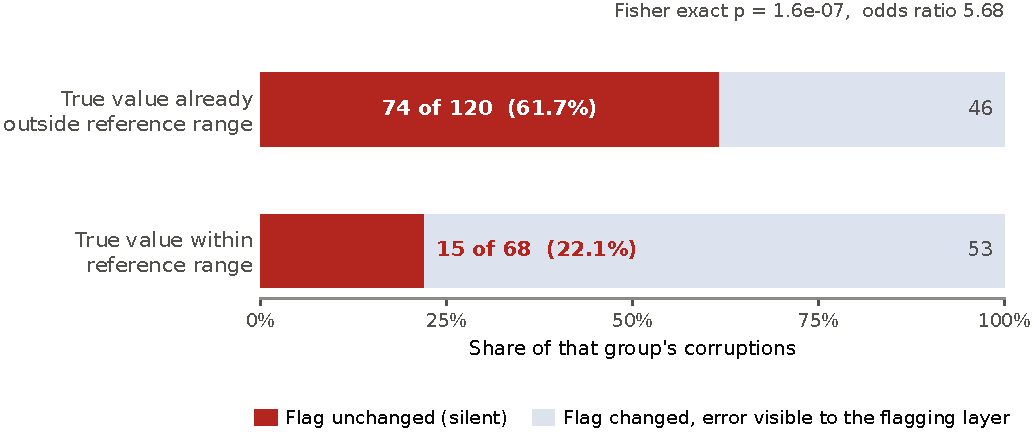
\includegraphics[width=0.92\textwidth]{figures/fig3_mechanism.pdf}
\caption{Corruption of a value that was already outside its reference range is far more likely
to leave the abnormality flag unchanged. Bars show, within each group, the share of that group's
corruptions that were silent. All 188 corruptions from Experiment~2 are included and the two
groups are disjoint.}
\label{fig:mechanism}
\end{figure}

Decimal-shift errors make the same point quantitatively. Of 188 corruptions, 102
(54.3\%) were decimal shifts, all of them upward. Tenfold shifts
($n = 87$) were silent in 42.5\% of cases, while hundredfold shifts ($n = 15$) were
silent in 86.7\%. The larger error is the more invisible one.

Troponin I illustrates the consequence. Fourteen of its fifteen corrupted readings were
hundredfold overstatements, and every one retained the \emph{Critical} flag:
0.07~ng/mL read as 7.0, 0.82 read as 82.0. A
borderline result and a result two orders of magnitude higher are indistinguishable downstream.

\subsection{A plausibility bound helps, and fails systematically}

The plausibility bound rejected 104 of the 188 corruptions (55.3\%) and rejected
none of the 636 correct values. The absence of false positives is guaranteed by the generator,
which samples truth values strictly inside the envelope, and is not an estimate of a real
false-positive rate.

Of the 89 silent corruptions, the bound recovered 33 (37.1\%), leaving 56 that
neither the flagging layer nor the plausibility check would surface.

Per-analyte detection ranges from 96.9\% for potassium to zero for troponin I,
ferritin, fasting glucose and eGFR (Table~\ref{tab:peranalyte}). We tested whether detection is
predicted by the ratio of plausible envelope width to reference range width. The association is
in the expected direction and does not reach significance at this sample size
(Spearman $\rho = -0.48$, $p = 0.09$, $n = 13$), and eGFR contradicts it: its envelope is the
narrowest of the panel relative to its reference range, yet no corruption was detected, because
the envelope's lower bound is zero and every observed eGFR corruption moved the value downward.
Detectability depends on where a corrupted value lands relative to an envelope boundary, which
is not captured by width alone.

\begin{table}[t]
\centering
\caption{Plausibility-bound detection rate per analyte, over the corruptions observed for that
analyte in Experiment~2. Analytes whose plausible envelope is wide relative to their reference
range, or whose envelope is open at the relevant end, are not protected.}
\label{tab:peranalyte}
\small
\begin{tabular}{lcc}
\toprule
Analyte & Corruptions & Detected (\%) \\
\midrule
Potassium          & 32 & 96.9 \\
Haemoglobin        & 33 & 90.9 \\
Sodium             & \phantom{0}6 & 83.3 \\
Platelets          & 16 & 75.0 \\
HbA1c              & \phantom{0}4 & 75.0 \\
Creatinine         & 27 & 59.3 \\
Blood urea nitrogen & \phantom{0}7 & 42.9 \\
White cell count   & 18 & 16.7 \\
LDL cholesterol    & \phantom{0}8 & 12.5 \\
eGFR               & \phantom{0}8 & \phantom{0}0.0 \\
Fasting glucose    & \phantom{0}8 & \phantom{0}0.0 \\
Ferritin           & \phantom{0}6 & \phantom{0}0.0 \\
Troponin I         & 15 & \phantom{0}0.0 \\
\bottomrule
\end{tabular}
\end{table}

\subsection{A language model extractor repaired nothing}
\label{sec:llm-extractor}

We replaced the deterministic parser with a language model extractor (Llama 3.2 3B via Ollama,
temperature 0) and ran both over identical OCR text across 12 conditions at two repeats. In
four of the 24 runs the model returned no values at all after emitting malformed JSON
(\texttt{rotate\_5.0} twice, \texttt{noise\_30} twice). Over the 260 readings from the 20 runs
that returned values, both extractors were correct on the same 188: zero repairs and zero new
errors.

The corruption is established before either extractor sees the text, and a model reading the
same damaged characters reproduces the same damaged number.

\section{Experiment 3: can a better reader fix it?}

Experiments~1 and 2 establish that the corruption happens and that the flagging layer cannot
see it. The obvious response is to read the page better. Experiment~3 tests that response
directly, including the approach a machine learning practitioner would reach for first, which is
to fine-tune the recogniser on in-domain data.

\subsection{Test sets}

\textbf{Test A} is the document and the 64 degradation runs of Experiment~1, giving 832 values.
It measures performance on the material the system was studied on.

\noindent \textbf{Test B} is held out. It comprises 20 further synthetic reports, 1{,}988 values, 12 to 18
analytes each, drawn across four column layouts and four laboratory identities, and rendered in
\textbf{Times and Courier}. Neither font appears anywhere in the fine-tuning data. Each report
is degraded under seven conditions: 300, 150, 120 and 100~dpi, an office scan, a phone
photograph and a poor fax. Test B exists to detect a model that has learned the study document
rather than the task.

The fine-tuning corpus is generated with random values, so no test value can have been
memorised.

\subsection{Readers compared}

\begin{itemize}
\item \textbf{Stock Tesseract 5.5} (\texttt{tessdata\_fast}), the pipeline measured above.
\item \textbf{Tesseract best} (\texttt{tessdata\_best}, float LSTM), the base for fine-tuning.
\item \textbf{Rescale variants} of both, in which the page is upscaled to at least 300~dpi by
Lanczos resampling before recognition, with the source resolution estimated from page width.
\item \textbf{Fine-tuned v1} (\texttt{labnum}): \texttt{tessdata\_best} fine-tuned on 6{,}000
synthetic laboratory lines in sans-serif faces, rendered across 72--300~dpi with blur, noise,
JPEG compression and rotation.
\item \textbf{Fine-tuned v2} (\texttt{labnum2}): the same recipe on 8{,}000 lines spanning
sans-serif, serif and monospace families, still excluding Times, Courier and Georgia.
\item \textbf{PP-OCR} via RapidOCR and ONNX Runtime. Both its detector and its
recogniser are unrelated to Tesseract, so it serves as an independent second reader.
\item \textbf{Qwen2.5-VL 3B} through Ollama, prompted for verbatim transcription, run on a
subset of conditions.
\end{itemize}

Fine-tuning follows the standard \texttt{tesstrain} recipe. Training lines are generated
programmatically as single-row laboratory entries with the analyte name, a sampled value, its
unit and its printed reference range, rendered at a resolution drawn from 72--300~dpi and
degraded with the same blur, noise, JPEG and rotation operators used in the evaluation
conditions. Version~1 used 6{,}000 lines in sans-serif faces only; version~2 used 8{,}000 lines
spanning sans-serif, serif and monospace families, excluding Times, Courier and Georgia so that
the held-out faces remain unseen. Values are sampled at random within each analyte's plausible
envelope, so no specific test value can have been memorised, though the analyte catalogue,
reference ranges and number formatting are shared with the test generator (see Limitations).

Line images with word-string box files are converted to \texttt{.lstmf} training records, and
\texttt{lstmtraining} then continues from the stock English LSTM at a learning rate of
$10^{-4}$ for 10{,}000 iterations before stopping. The base model is \texttt{tessdata\_best}. No early
stopping or validation-based checkpoint selection was used; the final iteration is the released
model. The resulting model is 15~MB and runs at the same speed as the stock float model.
Recognition uses page segmentation mode 6 throughout, matching Experiments~1 and 2, and the
training logs for both versions are released with the code.

\subsection{Analysis}

Experiment~2 argued that analytes read from one page are not independent observations. The same
argument applies here, so every comparison below treats the \emph{document} as the experimental
unit: exact value accuracy is computed within each of the 20 held-out reports and summarised
across them, dispersion is the standard deviation between documents, and engines are compared by
Wilcoxon signed-rank test over the 20 paired documents. Pooled counts are reported only for
corruption totals, where the quantity of interest is the count itself.

\subsection{Results}

Table~\ref{tab:engines} reports exact value accuracy by reader, and Figure~\ref{fig:engines}
shows the per-document distributions.

\begin{table}[t]
\centering
\caption{Exact value accuracy on the 20 held-out reports of Test~B, computed per document and
summarised across them, with the pooled low-resolution figure from Test~A for reference.
\emph{Silent} is the share of that reader's corruptions that preserved the abnormality flag,
which is the quantity the flagging layer cannot see.}
\label{tab:engines}
\small
\begin{tabular}{lccccc}
\toprule
Reader & Test B accuracy & SD between & $\leq$150~dpi & Corrupted & Silent \\
       & (mean of 20 docs) & documents & (Test A) & (of 1{,}988) & (\% of corruptions) \\
\midrule
Stock Tesseract 5.5      & 74.9\% & \phantom{0}5.7 & 60.0\% & 193 & 31.1\% \\
Tesseract best           & 73.0\% & \phantom{0}6.3 & 41.5\% & 204 & 26.5\% \\
Fine-tuned v2 + rescale  & 75.8\% & 10.5 & \textbf{100\%} & 268 & \textbf{37.7\%} \\
PP-OCR (RapidOCR)        & 78.0\% & \phantom{0}3.4 & 95.4\% & \textbf{\phantom{0}58} & 69.0\% \\
Stock + rescale          & 81.4\% & \phantom{0}2.7 & 98.5\% & 121 & 33.9\% \\
Tesseract best + rescale & \textbf{83.9\%} & \textbf{\phantom{0}1.4} & 92.3\% & \phantom{0}89 & 32.6\% \\
\bottomrule
\end{tabular}
\end{table}

\begin{figure}[t]
\centering
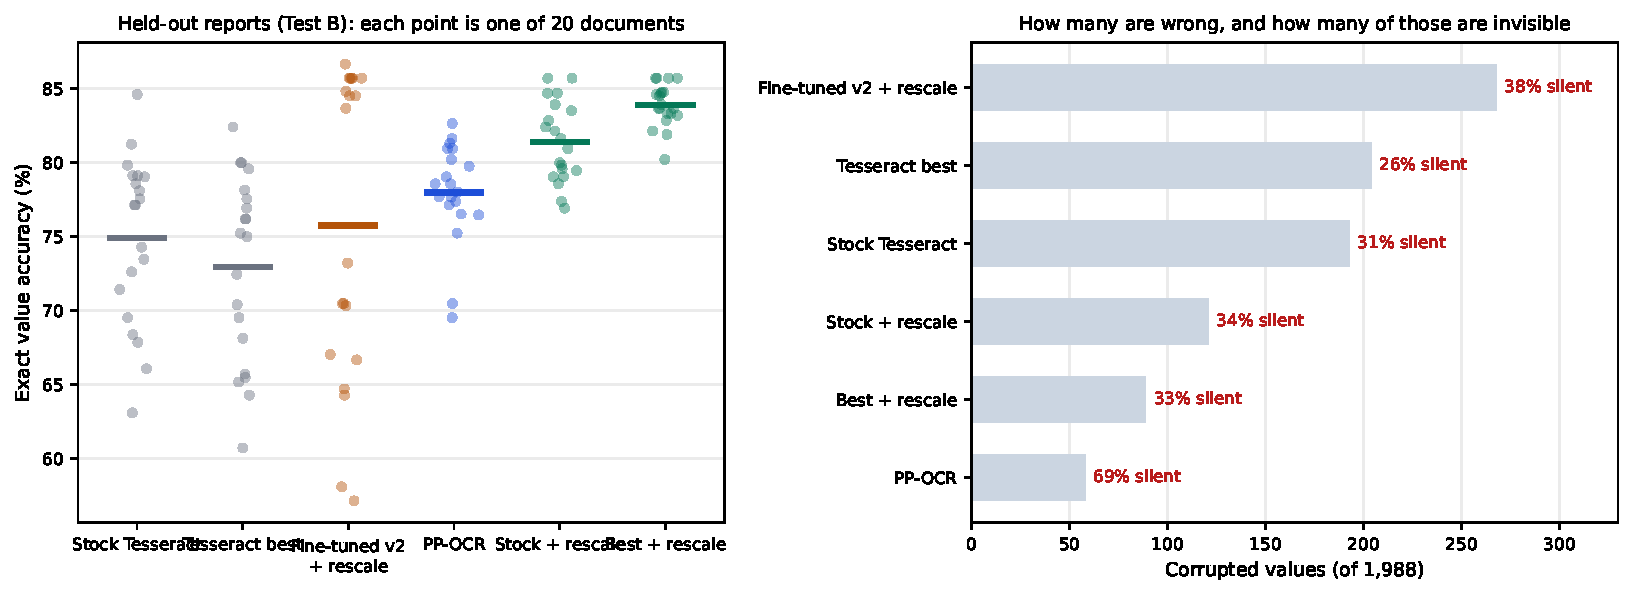
\includegraphics[width=\textwidth]{figures/fig4_engines.pdf}
\caption{Left: exact value accuracy on each of the 20 held-out reports, with the mean marked.
The fine-tuned model is both no more accurate on average than the stock model and far more
variable between documents. Right: how many values each reader got wrong, annotated with the
share of those errors that preserved the abnormality flag. PP-OCR makes the fewest errors and
the largest proportion of its errors are invisible.}
\label{fig:engines}
\end{figure}

\subsubsection{Fine-tuning is not the remedy it appears to be}

Read only on Test~A, the fine-tuned model is the clear winner: all 65 values exact in the
resolution sweep at $\leq$150~dpi, where the stock pipeline reads 39 of 65 correctly (60.0\%).
That denominator deserves emphasis. The $\leq$150~dpi column covers five resolution conditions
on one document, so 65 readings in total, all sharing a single rendering and layout. It is the
most favourable comparison available to the fine-tuned model and the least independent.

On held-out reports it does not. Mean accuracy is 75.8\% against the stock model's 74.9\%, a
difference of 0.8 percentage points that a paired test over the 20 documents does not
distinguish from zero (Wilcoxon signed-rank, $p = 0.63$). It also produces more corrupted values
than the model it was built to improve (268 against 193), and a larger share of those
corruptions are silent (37.7\% against 31.1\%).

The between-document standard deviation is the more revealing number. The fine-tuned model
varies across documents with an SD of 10.5 percentage points, against 1.4 for the best rescaling
configuration. It is not merely no better on average; it is unpredictable, which for a clinical
pipeline is the worse property.

The failure is interpretable, and it is specific to typography. Test~B is evenly split, 10
reports in Times and 10 in Courier, which separates the two cases
(Table~\ref{tab:fonts}). The fine-tuned model is the best reader in the panel on unseen Times at
85.3\%, and the worst on unseen Courier at 66.3\%, against 84.4\% for the base model it was
built from under the same rescaling. It gains 1.9 percentage points on the serif face and loses
18.1 on the monospace one.

The mechanism is a word-segmentation artefact. In monospace text the inter-character gap around
a decimal point is as wide as a space, and a model trained only on proportional faces reads
Courier \texttt{7.8} as \texttt{7 . 8}, which the row parser truncates to 7.

Version~1 of the fine-tune, trained on sans-serif faces alone, exhibits this severely. Its
result files had not been retained, so we re-ran it on Test~B for this manuscript: it reads
unseen Times at 85.0\% and unseen Courier at 46.8\%, a gap of 38.2 percentage points, producing
482 corrupted values of which 288 are silent. Version~2 added serif and monospace families to
the training mix and halved the gap to 19.0 points, but did not remove it. The progression is
the clearest statement of the problem: adding font diversity to the training corpus reduces the
dependence on typography without eliminating it, while the configuration that never learned
typography at all shows no dependence.

\begin{table}[t]
\centering
\caption{Exact value accuracy on Test~B by typeface, 10 reports each. Neither face appears in
any fine-tuning corpus. Version~1 was trained on sans-serif faces only and version~2 added serif
and monospace families; the fine-tuned models are the only readers whose accuracy depends
strongly on which unseen face they meet, and the dependence shrinks as training typography
widens.}
\label{tab:fonts}
\small
\begin{tabular}{lccc}
\toprule
Reader & Times & Courier & Difference \\
\midrule
Stock Tesseract 5.5      & 71.0\% & 78.8\% & $-7.8$ \\
Tesseract best           & 67.8\% & 78.0\% & $-10.2$ \\
Fine-tuned v1 + rescale  & 85.0\% & \textbf{46.8\%} & $\mathbf{+38.2}$ \\
Fine-tuned v2 + rescale  & \textbf{85.3\%} & 66.3\% & $+19.0$ \\
PP-OCR (RapidOCR)        & 78.4\% & 77.4\% & $+1.0$ \\
Stock + rescale          & 83.0\% & 79.9\% & $+3.1$ \\
Tesseract best + rescale & 83.4\% & 84.4\% & $-1.0$ \\
\bottomrule
\end{tabular}
\end{table}

\subsubsection{Upscaling the page is the single largest gain}

Rescaling to at least 300~dpi before recognition requires no training, no new model and no
change of engine. Over the 20 held-out documents it improves the stock model by 6.5 percentage
points ($p = 0.0012$) and \texttt{tessdata\_best} by 9.0 points relative to stock
($p = 0.0001$), and it beats the fine-tuned model by 8.1 points ($p = 0.031$). It takes
low-resolution accuracy on Test~A from 60.0\% to 98.5\% and reduces decimal-point losses on
Test~B from 109 to 11.

The reason is mechanical rather than statistical. A decimal point at 100~dpi occupies a handful
of pixels and the recogniser's line model has little evidence to work with. Upscaling adds no
information, but it presents the information already present at a scale the model was trained
for. It also cannot overfit, because it introduces no parameters.

\subsubsection{The vision--language model rewrites rather than reads}

The vision--language model was run on a subset of conditions, so it is reported separately
(Table~\ref{tab:vlm}) and compared against the stock pipeline on exactly the same document and
condition cells.

\begin{table}[t]
\centering
\caption{Qwen2.5-VL 3B against the stock pipeline on identical cells. The Test~B subset covers
only three conditions, none of which is the poor-fax condition on which the model's
characteristic failure was observed, so the 100\% figure should not be read as a general result.}
\label{tab:vlm}
\small
\begin{tabular}{lcccc}
\toprule
 & Cells & Conditions & Qwen2.5-VL exact & Stock exact \\
\midrule
Test A & 260 & 12 of 64 & 85.0\% & 59.2\% \\
Test B & 339 & 3 of 7 (300~dpi, 100~dpi, phone photo) & 100\% & 82.6\% \\
\bottomrule
\end{tabular}
\end{table}

Where the page is legible the model transcribes more accurately than any other reader tested,
and it never dropped a decimal point. On fax-quality pages its behaviour changes in kind rather
than degree. Instead of emitting a garbled token or no value, it produces fluent, well-formed
values that are not printed on the page, and the substitutions move results toward the normal
range: HbA1c 9.2 returned as ``5.2 \%, range 4.5--5.8, N''; haemoglobin 9.4 flagged \emph{Low}
returned as 13.4; potassium 5.8 flagged \emph{High} returned as 3.6 with an invented unit and
reference range. It also invented flags on clean pages and converted g/dL to g/L.

Every one of these passes a physiological plausibility check, because the values are
physiologically ordinary. This is a worse failure mode than a dropped decimal point: a lost
decimal produces an implausible number that a bound can catch, whereas an invented normal value
is indistinguishable from a correct one by any check that inspects the value alone. The
direction compounds the problem, since values are moved toward normality and therefore away from
attention. Governance layers have been reported to reduce hallucination rates substantially in
document extraction pipelines \citep{sediqin2026sage}, which is consistent with our finding that
the remedy is external verification rather than a better model.

\subsection{A taxonomy of what actually goes wrong}

Across both test sets the errors fall into five mechanisms.

\begin{enumerate}
\item \textbf{Lost decimal point.} At low resolution the separator disappears: creatinine
2.1 read as 21, white cell count 7.4 read as 74. The decimal in the printed reference range
disappears with it (``0.6--1.2'' becomes ``06--12''), so value and range shift together and a
row-local consistency check cannot detect the change.
\item \textbf{Range fall-through.} When the result cell is illegible, a parser that takes the
first number on the line falls through to the lower bound of the reference range: INR 1.1 read
as 0.8, glucose 77 read as 70.
\item \textbf{Digit substitution.} 31 read as 32, 195 as 198, 121 as 127. Plausible, same flag,
invisible to any rule.
\item \textbf{Split decimal.} A monospace decimal point read as a word break, so
\texttt{7.8} becomes \texttt{7 . 8} and the parser truncates to 7. Introduced by the
fine-tuned models and absent from every stock configuration (Table~\ref{tab:fonts}).
\item \textbf{Generative rewriting.} Produced only by the vision--language model.
\end{enumerate}

Mechanisms 1, 2 and 4 have structural signatures that a checker can exploit. Mechanisms 3 and 5
do not, and require a second opinion.

\section{Experiment 4: what catches the errors that remain}

No reader in Table~\ref{tab:engines} avoids undetected errors across all conditions.
Experiment~4 therefore tests
verification rather than recognition. Nothing is corrected automatically; a failed check routes
the value to human review against the source image, which is the only safe action when the
system cannot tell which of two readings is right.

Terms are used precisely below. A value is \emph{corrupted} if the reader emitted a number that
differs from truth. A check \emph{catches} a value by routing it to human review; nothing is
corrected automatically, and a caught value is not a corrected value. A \emph{false alarm} is a
correct value routed to review. The \emph{review rate} is the share of all extracted values a
human would inspect, and \emph{undetected wrong} values are corrupted values the system accepted
without review. The denominators differ by test set: 619 of 832 values were extracted at all on
Test~A, of which 43 were corrupted; 1{,}685 of 1{,}988 were extracted on Test~B, of which 193
were corrupted. Values that were never extracted are absences the caller can observe and are
excluded from these counts.

Four checks are layered on the existing plausibility bound. The \emph{precision} check flags a
value printed without a decimal for an analyte that laboratories always report with one. The
\emph{magnitude} check flags a value far above its plausible window where division by a power of
ten would fit, restricted to the high side and to narrow-range analytes so that genuine extremes
such as troponin in infarction are not flagged. The \emph{structure} check detects range
fall-through by testing whether the extracted number is immediately followed by a range
separator and a second number. The \emph{agreement} check requires a second, independently built
reader to return the same value.

The claim that the two readers are independent is architectural rather than statistical, and it
the distinction matters. Tesseract recognises a segmented text line with
a recurrent LSTM over the whole line; PP-OCR detects text regions with a separate convolutional
detector and recognises each crop independently, through a different training corpus and a
different inference stack. They therefore fail on different inputs: Tesseract's characteristic
error is losing a small separator within a line it has segmented correctly, while PP-OCR's is a
detection boundary that clips or merges fields. Our data are consistent with this, since the two
readers' error sets overlap only partially. What we have not established is statistical
independence of their errors, which would require a failure model neither engine provides. Both
could in principle fail identically on a sufficiently degraded page, and in that case agreement
would confirm a wrong value rather than catch it. The check therefore reduces the chance of an
undetected error; it does not eliminate it.

\begin{table}[t]
\centering
\caption{Verification performance, with stock Tesseract as the primary reader and PP-OCR as the
second. \emph{Wrong caught} is the number and share of corrupted values routed to review on
Test~B, with an exact binomial 95\% confidence interval; \emph{false alarms} is the share of
correct values routed to review; \emph{review rate} is the total share of values a human would
inspect. Silent counts are from Test~A. No clinician reviewed any output and no clinical
decision was simulated: routing to review is a property of the software, not a measured
improvement in care.}
\label{tab:verify}
\small
\begin{tabular}{lccccc}
\toprule
Checks & Silent caught & Wrong caught $\cdot$ B & 95\% CI & False alarms & Review rate \\
       & $\cdot$ A & (of 193) & & $\cdot$ B & $\cdot$ B \\
\midrule
None                              & \phantom{0}0 / 28 & \phantom{00}0 \phantom{0}(0.0\%) & \phantom{0}0.0--1.9 & 0.0\% & \phantom{0}0.0\% \\
Plausibility only (existing)      & \phantom{0}9 / 28 & \phantom{0}99 (51.3\%) & 44.0--58.5 & 0.8\% & \phantom{0}6.6\% \\
\quad + precision                 & 23 / 28 & 158 (81.9\%) & 75.7--87.0 & 0.8\% & 10.1\% \\
\quad + precision + structure     & 23 / 28 & 168 (87.0\%) & 81.5--91.4 & 0.9\% & 10.7\% \\
\quad + agreement with PP-OCR     & \textbf{28 / 28} & \textbf{193 (100\%)} & \textbf{98.1--100} & 9.4\% & 19.8\% \\
\bottomrule
\end{tabular}
\end{table}

The structural checks are nearly free: they raise detection from 51.3\% to 87.0\% while
increasing false alarms by 0.1 percentage points. Agreement with a structurally different reader
closes the remainder, at the cost of routing roughly one value in five to review. With agreement
enabled, every value the system accepted in both test sets was correct. The result holds when
the fine-tuned model is the primary reader, where agreement still catches 266 of 268 wrong
values on Test B.

The practical reading is that the second reader is doing work no single reader can do for
itself, because the errors that survive the structural checks are precisely the ones that look
normal.

The review burden translates as follows. At the structural tier, 10.7\% of
values are routed to review and 87.0\% of wrong values are caught: for a clinic ingesting 100
reports a day with a 14-analyte panel, that is roughly 150 values to check against the source
image. Adding the agreement check raises the catch rate to 100\% and the burden to 19.8\%, or
roughly 280 values a day. Those are very different operational propositions, and the choice
between them is not a technical one. It depends on document quality, on staffing, and on what
the values are used for. What the data establish is the shape of the trade: the first 87\% of
errors are nearly free, and eliminating the remainder costs roughly a doubling of review
volume.

\section{Discussion}

The practical consequence is that character-level accuracy does not bound value-level risk in a
pipeline of this shape. A system reporting 88.9\% character accuracy was delivering
wrong values for roughly a third of the panel, and for nearly half of those the downstream
alerting layer could not tell.

Threshold quantisation is common in clinical software, because reference ranges and severity
bands are how laboratory results are presented. The finding here is that quantisation is also an
information-destroying step placed immediately after an error-prone one. Any check that operates
on the flag rather than the value inherits a blind spot whose size depends on how abnormal the
true value was. The patients whose values are furthest outside the reference range are the
patients whose corrupted readings are hardest to detect.

The plausibility bound is worth implementing and is not sufficient on its own. It is cheapest
where it is least needed, for analytes like potassium whose physiological envelope is narrow,
and it provides nothing for analytes like troponin whose plausible range spans several orders of
magnitude.

One distinction in the results carries directly into how such a system should be read. An
unread analyte is an absence the caller can notice; a misread one is a confident wrong answer.
Pooling them, as a single extraction-failure rate would, conceals the difference between a
failure that announces itself and one that does not.

Experiments~3 and 4 bear on how such a pipeline should be built. The instinct to fix a reading
problem by training a better reader is, on our data, actively misleading. Evaluated on the
document it was tuned for, the fine-tuned recogniser reads perfectly in the failure regime; the
same model is no better than stock on held-out reports and produces more silent corruptions
than the model it replaced. A practitioner who held out no unseen typography would have
concluded the problem was solved and deployed a model that fails differently rather than less.

By contrast, the intervention that worked is not a model at all. Upscaling the page before
recognition improves low-resolution accuracy more than any model change we tested, requires no
training data, and cannot overfit, because it adds no parameters. When a failure is caused by
information being presented at the wrong scale, the appropriate remedy is to change the scale.

The vision--language result deserves separate emphasis for clinical readers. Such models are
increasingly proposed for document understanding, and on legible pages this one was the most
accurate reader we tested. Its failure mode on illegible pages is not noise but confabulation,
and the invented values moved toward the normal range. A system that silently normalises
abnormal results is more dangerous than one that fails loudly, and conventional accuracy
reporting would have recorded this model as the best performer.

The pattern across these experiments is that undetected error is reduced by disagreement rather
than by accuracy. Two readers built on different principles fail on different inputs, and requiring them
to agree converts an undetectable error into a detectable one. On our data that reduced
undetected wrong values to zero, at a review burden of roughly one value in five. Whether that
burden is acceptable is a deployment question that depends on volume and on what the values are
used for.

\section{What follows for a system that reads clinical documents}

The findings suggest five things a team building such a pipeline could act on. We state them as
implications of the mechanism rather than as validated interventions, since none has been tested
in a clinical setting.

\begin{enumerate}
\item \textbf{Do not report character accuracy as a safety figure.} It did not bound value-level
error anywhere in our data, and the gap was widest in the degradation regime real documents
occupy. Report the share of target values extracted exactly, which is the quantity the clinical
logic consumes.

\item \textbf{Normalise resolution before recognition.} Upscaling to at least 300~dpi gave a
larger improvement than any model change we tested, adds no parameters and cannot overfit. It is
a few lines of code at the front of the pipeline.

\item \textbf{Hold out typography before trusting a fine-tuned recogniser.} Evaluated only on
familiar documents, our fine-tuned model looked like a solution. On fonts it had never seen it
was no better than stock and produced more invisible errors. A held-out set in a deliberately
different typeface separates those two conclusions and costs a few hours to build.

\item \textbf{Treat a generative reader's output as a claim, not a transcription.} The
vision--language model was the most accurate reader on legible pages and, on illegible ones,
produced plausible values that were not printed, biased toward the normal range. Any pipeline
using such a model needs its output checked against a deterministic reader on the same region,
because the failure is invisible to checks that inspect the value alone.

\item \textbf{Carry the distance, not just the side, of a threshold.} The flag is where the
information is lost. A system that retains how far a value lies outside its reference range, or
that compares against the range printed on the document rather than a hardcoded one, can detect
errors that a flag cannot represent.
\end{enumerate}

Of these, the second and third cost almost nothing and we would expect them to generalise. The
fifth is a design change with wider consequences and would need evaluating in context.

\section{Limitations}

The documents are synthetic. They carry exact ground truth, which is what makes the measurement
possible, and they are not real clinical documents. Nothing here establishes a rate for any
deployed system, and no clinician reviewed any output.

One OCR engine was used, at one page segmentation mode, with one document layout and one panel
of 13 analytes. Every quantity we report is conditional on that stack.

Resolution and pixels per glyph are entangled, since body text varies between 8.5 and 10 point
across the generated documents. A reader could reasonably hold that character size in pixels,
rather than nominal resolution, is the operative variable, and this design cannot separate them.

The plausibility envelope is our construction. Its zero false-positive rate is an artefact of a
generator that samples inside it.

The degradation sweep in Experiment~1 and the extractor comparison use a single document. Only
the resolution sweep is replicated across 10 documents, and only the resolution results carry
between-document dispersion.

We did not measure whether a corrupted value changes a clinical recommendation. The propagation
of a corrupted value into generated text was observed on one document and is not quantified
here.

The held-out set in Experiment~3 is held out with respect to typography, layout and values, but
not with respect to the generator. Test~B and the fine-tuning corpus are produced by the same
code and therefore share an analyte catalogue, a set of reference ranges, and the conventions by
which numbers and ranges are formatted. A fine-tuned model could in principle exploit those
shared conventions in a way it could not exploit a real laboratory's. This makes our held-out
result conservative in one direction, since the fine-tuned model failed to generalise even on
material that shares its generator, and optimistic in another, since we cannot measure how it
would behave on genuinely foreign report conventions. Test~B is also still synthetic and rendered
digitally before degradation. Real scans add skew, shadows,
staples, stamps, handwritten annotations and photocopying artefacts that our degradation model
does not reproduce. The held-out comparison therefore tests generalisation across fonts and
layouts, not across capture devices.

One vision--language model was evaluated, at 3 billion parameters, running locally, on a subset
of conditions. Larger models read more accurately. We cannot say from our data whether the
rewriting behaviour diminishes with scale, and we did not test that.

The analyte conventions underlying the precision and magnitude checks, meaning which tests are
conventionally printed with a decimal and what counts as a narrow range, are typical adult
values assembled for this study rather than a clinical standard. A deployment would take them
from the laboratory's own information system.

The review rate reported for the agreement check is measured on our degradation distribution. A
document population with better average capture quality would produce fewer disagreements and a
lower burden, and a worse one would produce more.

\section{Conclusion}

Character accuracy and value accuracy come apart under degradation, and the gap is widest
exactly where the clinical stakes are highest. Nearly half of the value corruptions we observed
preserved the abnormality flag, and corruption of an already-abnormal value was 2.80 times as
likely to be silent as corruption of a normal one (95\% CI 1.75--4.47), because a threshold
cannot represent how far past it a value has moved. A plausibility bound recovers some of this and fails
systematically for the analytes with the widest physiological ranges. Substituting a language
model for a deterministic parser changed nothing, because the information was lost before either
could read it. Knowing where a number came from is not the same as knowing it was read
correctly.

Attempting to fix this by training a better recogniser produced a model that reads the document
it was tuned for perfectly and unseen typography worse than the model it replaced, while
increasing the number of corruptions the alerting layer cannot see. Upscaling the page before
recognition, which adds no parameters and cannot overfit, did more for low-resolution accuracy
than any model we trained. A vision--language model read legible pages better than anything else
and, on illegible pages, invented plausible values in the direction of normality. What most reduced undetected errors was none of these: it was requiring two independently built readers to agree, which
left no undetected wrong value in either test set, within the limits that a finite sample with
zero observed failures can establish. In a pipeline that reduces measurements to
flags, the useful question is not how accurately the page was read, but whether anything
downstream would notice if it had not been.

\section*{Data and code availability}

\ifanon
All materials are provided through an anonymised repository link with the submission.
\else
All materials are available at
\url{https://github.com/thejabirhussain/silent-corruption-clinical-ai}, released under an open
licence. The repository contains the document generator and the truth files it writes, the
degradation and recognition harness, the fine-tuning scripts and training logs for both model
versions, the per-reading result tables from which every number in this paper is computed, the
verification implementation, and the scripts that produce each figure and table. Reproduction
instructions, including the exact commands for generating the held-out test set, training a
model and evaluating any reader in Table~\ref{tab:engines}, are in the repository README.

The fine-tuned Tesseract models are 15~MB each and are released with the code. Third-party
components are obtained from their own distributions rather than redistributed: the stock
Tesseract models from the \texttt{tessdata} and \texttt{tessdata\_best} repositories, PP-OCR
through \texttt{rapidocr\_onnxruntime}, and Qwen2.5-VL 3B through Ollama.
\fi

Synthetic data are used throughout. No real patient information was processed at any stage, and
no component of the released material contains or derives from patient data.

\section*{Ethics approval}

This study required no ethical approval and none was sought. It uses only synthetic laboratory
reports generated programmatically for this work. No human subjects, human tissue, identifiable
personal data or real clinical records were involved at any stage, and no participant
identifying information appears in the manuscript or in the released materials.

\section*{Author contributions}

M.J.H.S.\ is the sole author. He conceived the study, designed and implemented the experiments,
generated the synthetic corpora, fine-tuned and evaluated the recognition models, implemented
the verification layer, performed the statistical analysis, produced the figures and wrote the
manuscript. The clinical decision support prototype whose extraction path is measured here was
also built by the author, as an unfunded academic project.

\section*{Funding}

This research received no specific grant from any funding agency in the public, commercial or
not-for-profit sectors.

\section*{Competing interests}

The author declares no competing interests. Neither the author nor the author's institution has
received payments or services from any third party related to this work in the past 36 months.
The clinical decision support prototype measured in this study was built by the author as an
unfunded academic project and is not a commercial product.

\section*{Use of artificial intelligence}

The author used Anthropic Claude as a coding assistant, to help write and debug the experiment
and analysis code, and to help draft and check the manuscript text. The research question,
experimental design, execution, analysis and interpretation are the author's own. The author
reviewed and edited all content, verified every reported value against the released result
files, and takes full responsibility for this manuscript.

\begin{thebibliography}{99}
\small

\bibitem[Amugongo et al.(2025)]{amugongo2025rag}
Amugongo, L. M., et al. (2025).
Retrieval augmented generation for large language models in healthcare: a systematic review.
\emph{PLOS Digital Health}, 4(6), e0000877.

\bibitem[Ben Abacha and Demner-Fushman(2019)]{benabacha2019medquad}
Ben Abacha, A., and Demner-Fushman, D. (2019).
A question-entailment approach to question answering.
\emph{BMC Bioinformatics}, 20, 511.

\bibitem[Yu et al.(2026)]{yu2026benchmark}
Yu, A., Weile, J., and Courtot, M. (2026).
Benchmarking LLM-based information extraction tools for medical documents.
\emph{medRxiv}, 2026.01.19.26344287.
\url{https://doi.org/10.64898/2026.01.19.26344287}

\bibitem[Collins et al.(2024)]{collins2024tripodai}
Collins, G. S., Moons, K. G. M., Dhiman, P., et al. (2024).
TRIPOD+AI statement: updated guidance for reporting clinical prediction models that use
regression or machine learning methods.
\emph{BMJ}, 385, e078378.

\bibitem[Gao et al.(2023)]{gao2023rag}
Gao, Y., et al. (2023).
Retrieval-augmented generation for large language models: a survey.
\emph{arXiv:2312.10997}.

\bibitem[Kilickaya et al.(2014)]{kilickaya2014ranges}
Kilickaya, O., Schmickl, C., Ahmed, A., Pulido, J., Onigkeit, J., Kashani, K., Gajic, O.,
Herasevich, V., and Pickering, B. (2014).
Customized reference ranges for laboratory values decrease false positive alerts in intensive
care unit patients.
\emph{PLoS ONE}, 9(9), e107930. \url{https://doi.org/10.1371/journal.pone.0107930}

\bibitem[Hemmer et al.(2024)]{hemmer2024confidence}
Hemmer, A., Coustaty, M., Bartolo, N., and Ogier, J.-M. (2024).
Confidence-aware document OCR error detection.
\emph{arXiv:2409.04117}.

\bibitem[Lu et al.(2024)]{lu2024clinicalrag}
Lu, Y., Zhao, X., and Wang, J. (2024).
ClinicalRAG: enhancing clinical decision support through heterogeneous knowledge retrieval.
In \emph{Proceedings of the KnowLLM Workshop, ACL 2024}, pp. 64--68.

\bibitem[Sediqin et al.(2026)]{sediqin2026sage}
Sediqin, M., Dalmia, S., Thoppanahalli, S., Kovvuri, S. K. R., and Mukherji, A. (2026).
SAGE: governed artifact generation from enterprise guidelines.
\emph{arXiv:2609.17775}.

\bibitem[Smith(2007)]{smith2007tesseract}
Smith, R. (2007).
An overview of the Tesseract OCR engine.
In \emph{Ninth International Conference on Document Analysis and Recognition (ICDAR)},
pp. 629--633.

\bibitem[Wang et al.(2026)]{wang2026keycoverage}
Wang, Y., Li, Y., Qin, Y., and Qian, H. (2026).
Key coverage matters: semi-structured extraction of OCR clinical reports.
\emph{arXiv:2605.09440}.

\end{thebibliography}

\end{document}
